% Fragmento para integrar en el documento principal.
% Paquetes necesarios: \usepackage{graphicx}, \usepackage{listings}, \usepackage{hyperref}

\section{Actividad 2. Contenedores: de Dockerfile a despliegue}

\subsection{Contenedor nginx e imagen personalizada}
Se ejecutó \texttt{nginx:alpine} y se comprobó su página de bienvenida. Después se construyó una imagen con una página HTML propia. Para evitar interferencias con otros servicios se utilizaron los puertos locales 18082 y 18083, respectivamente.

\begin{lstlisting}[language=bash]
docker run -d -p 127.0.0.1:18082:80 --name sd-p05-nginx nginx:alpine
docker build -t sd-p05-web:v1 practicas/P05/actividad2/web
docker run -d -p 127.0.0.1:18083:80 --name sd-p05-web-estatica sd-p05-web:v1
\end{lstlisting}

El archivo \texttt{Dockerfile} de la página copia el HTML al directorio que nginx sirve por defecto:
\begin{lstlisting}
FROM nginx:alpine
COPY index.html /usr/share/nginx/html/index.html
\end{lstlisting}

\begin{figure}[htbp]
\centering
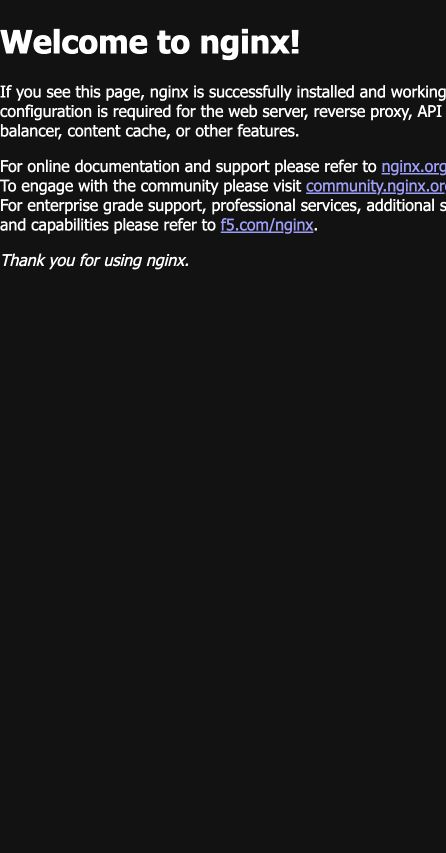
\includegraphics[width=.38\textwidth]{practicas/P05/evidencias/nginx-original.jpg}

\includegraphics[width=.38\textwidth]{practicas/P05/evidencias/nginx-personalizado.jpg}
\caption{Nginx original y página personalizada.}
\end{figure}

\subsection{Construcción en varias etapas}
Se compiló el mismo programa Go de dos maneras. En la primera, el compilador permanece en la imagen; en la segunda, se compila en una etapa y solo se copia el ejecutable a una imagen Alpine. Ambas mostraron el mismo mensaje al ejecutarse.

\begin{lstlisting}
FROM golang:1.24-alpine AS build
WORKDIR /src
COPY main.go .
RUN CGO_ENABLED=0 go build -ldflags="-s -w" -o /hola main.go
FROM alpine:3.21
COPY --from=build /hola /hola
CMD ["/hola"]
\end{lstlisting}

En la ejecución realizada, \texttt{docker images} mostró 433 MB para la imagen de una etapa y 14.8 MB para la de varias etapas. El tamaño depende de la arquitectura, la versión y las capas de las imágenes. También se consultaron la configuración, los registros y el consumo mediante \texttt{docker inspect}, \texttt{docker logs} y \texttt{docker stats}. Las salidas se conservaron en \texttt{evidencias/actividad2-salida.txt}.

\begin{figure}[htbp]
\centering
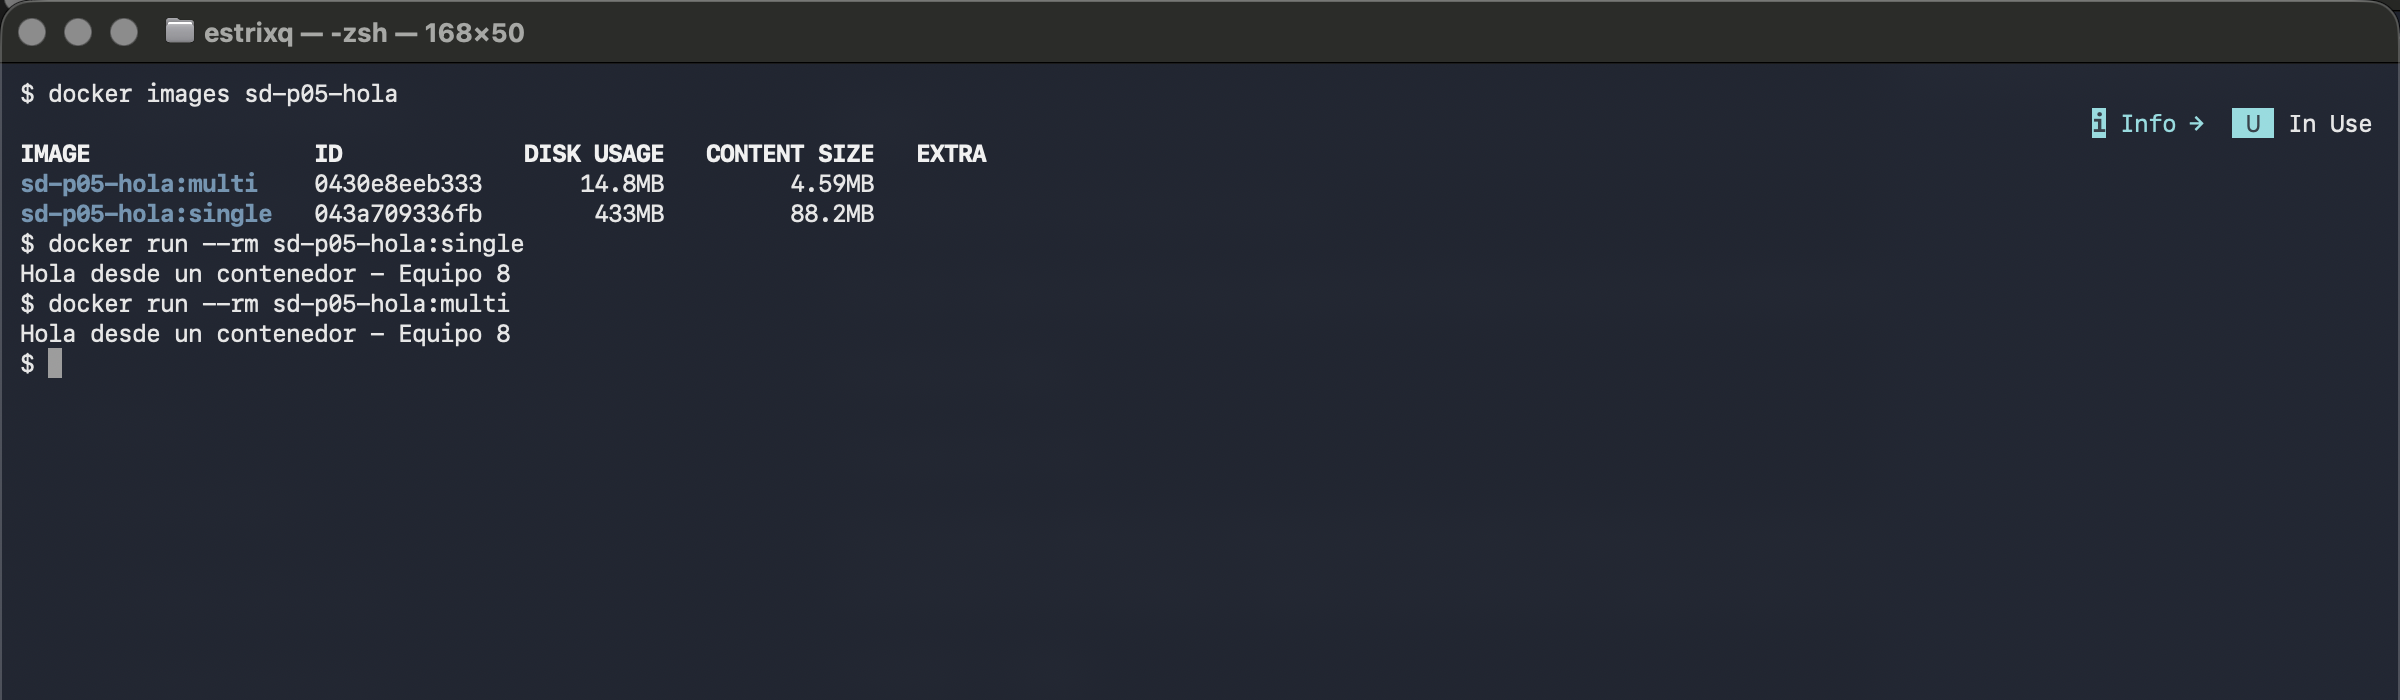
\includegraphics[width=\linewidth]{practicas/P05/evidencias/recortes/docker-imagenes.png}
\caption{Comparación de tamaños y ejecución de ambas imágenes.}
\end{figure}
\begin{figure}[htbp]
\centering
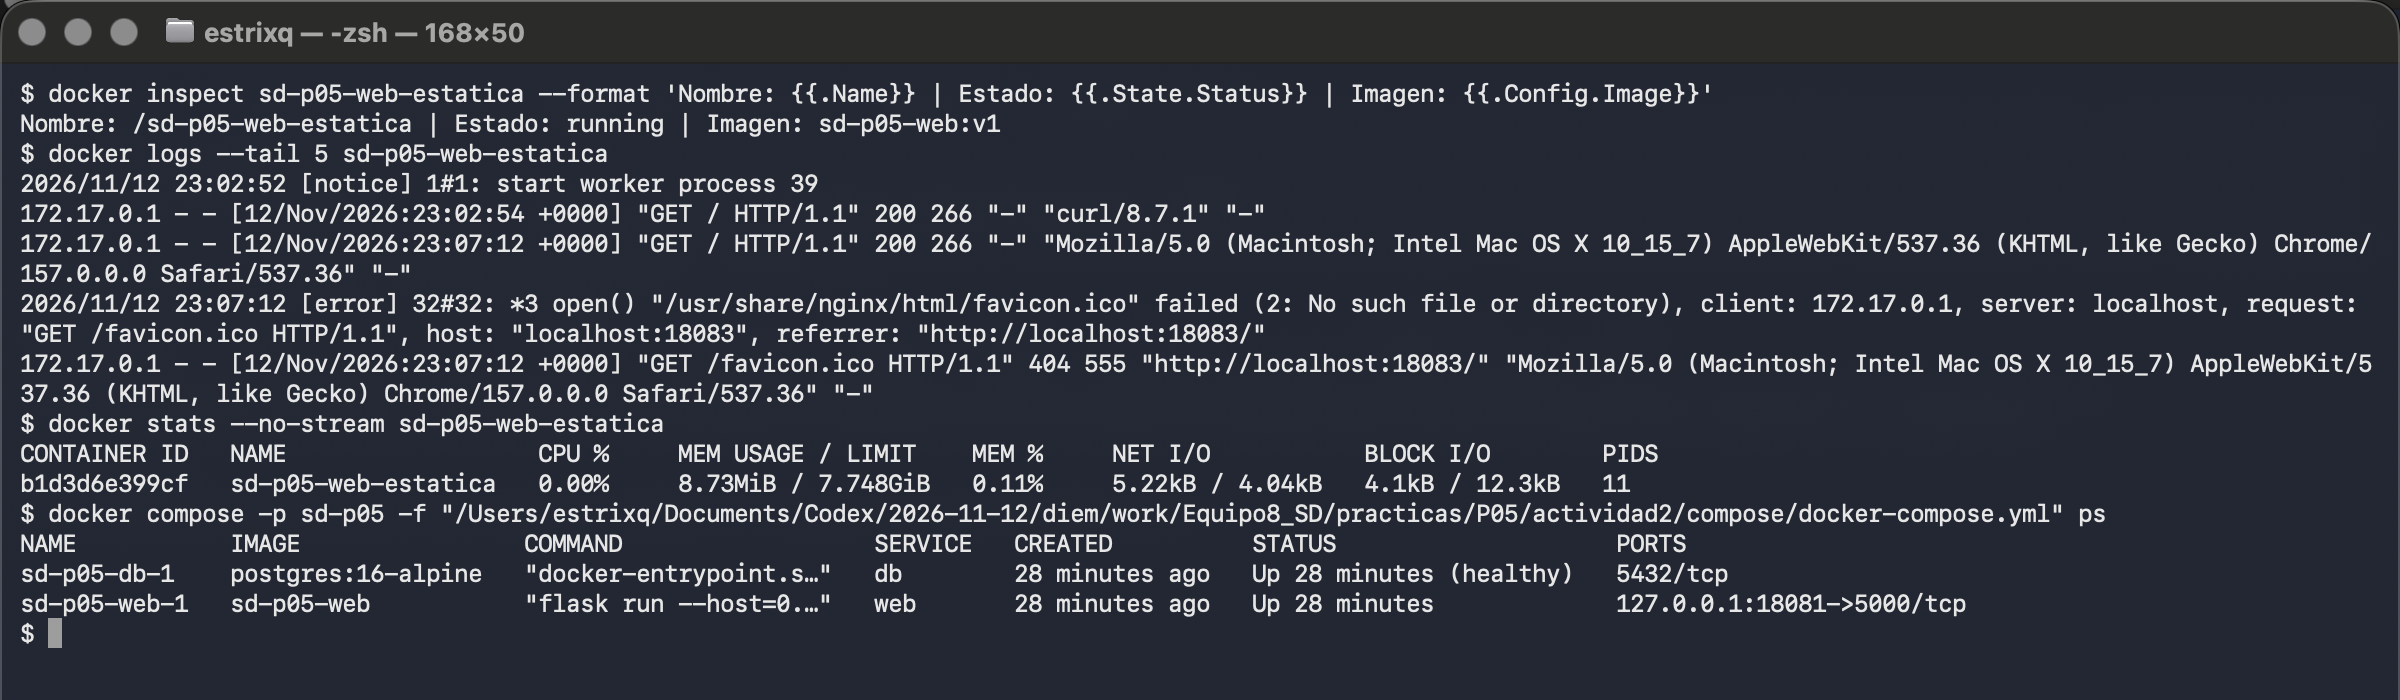
\includegraphics[width=\linewidth]{practicas/P05/evidencias/recortes/docker-inspeccion-compose.png}
\caption{Inspección, registros, consumo y servicios de Compose.}
\end{figure}

\subsection{Aplicación con Docker Compose}
Se construyó una aplicación Flask que se conecta a PostgreSQL mediante el nombre de servicio \texttt{db}. En cada visita inserta un registro y consulta el total almacenado. La base utiliza un volumen y una comprobación de salud; el servicio web espera a que esté lista. En dos solicitudes consecutivas se observaron los valores 1 y 2. El código completo está en \texttt{actividad2/compose}.

\begin{lstlisting}[language=bash]
docker compose -p sd-p05 -f practicas/P05/actividad2/compose/docker-compose.yml up -d --build
\end{lstlisting}

\begin{figure}[htbp]
\centering
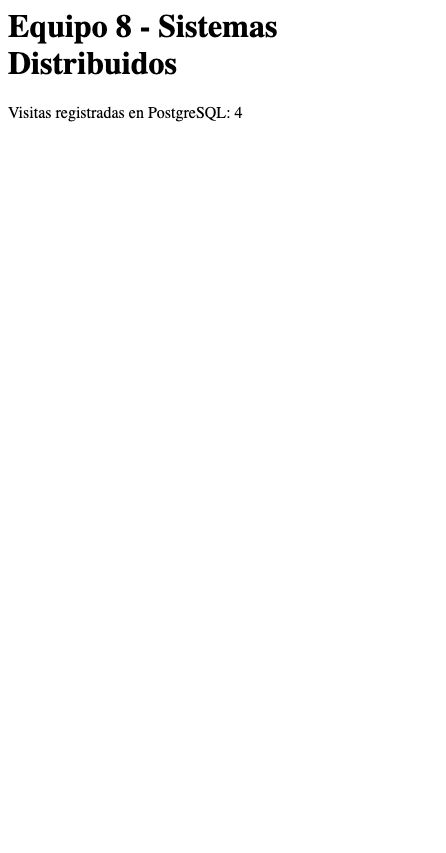
\includegraphics[width=.38\textwidth]{practicas/P05/evidencias/compose.jpg}
\caption{Aplicación Flask conectada a PostgreSQL.}
\end{figure}

\subsection{Preguntas de reflexión}
\begin{enumerate}
\item \textbf{Podman y rootless.} Ejecutar contenedores sin privilegios de administrador reduce las consecuencias de una vulnerabilidad, ya que el proceso y sus identificadores se limitan mediante espacios de nombres de usuario. Podman puede trabajar sin un daemon central. Docker Engine normalmente utiliza un daemon con privilegios elevados que administra imágenes y contenedores, aunque Docker también ofrece un modo rootless; no es correcto afirmar que siempre requiere root. En Docker Desktop sobre macOS, el motor Linux funciona dentro de una VM.
\item \textbf{Multi-stage y distroless.} Una imagen final que no incluye compiladores ni dependencias de construcción suele ser más pequeña y expone menos herramientas y componentes potencialmente vulnerables. Esto reduce la superficie de ataque, aunque no garantiza por sí solo la seguridad. Las imágenes distroless contienen la aplicación y sus dependencias de ejecución mínimas, generalmente sin gestor de paquetes ni shell; esto reduce componentes que mantener y analizar.
\item \textbf{Red de Compose.} Compose crea una red para el proyecto y registra los nombres de los servicios en el DNS interno. Así, \texttt{web} resuelve \texttt{db} a la dirección del contenedor de PostgreSQL y se conecta al puerto 5432 sin publicar ese puerto en el anfitrión.
\end{enumerate}

\section{Actividad 3. Orquestación con Kubernetes}

\subsection{Despliegue y escalado}
Se creó un clúster local Kind de un nodo con un archivo de configuración independiente. Se aplicó un Deployment de nginx con dos réplicas y un Service NodePort. El puerto del nodo 30080 se mapeó al 18080 del equipo; se comprobó que la página de nginx respondía en \texttt{localhost:18080}. Al aumentar a cinco réplicas se observaron cinco pods en estado \texttt{Running} en el único nodo. Posteriormente se redujo a una réplica y se observó la terminación de las demás.

\begin{lstlisting}[language=bash]
kubectl apply -f deployment.yaml -f service.yaml
kubectl get nodes
kubectl get pods,service -o wide
kubectl scale deployment mi-app --replicas=5
kubectl scale deployment mi-app --replicas=1
\end{lstlisting}

\begin{figure}[htbp]
\centering
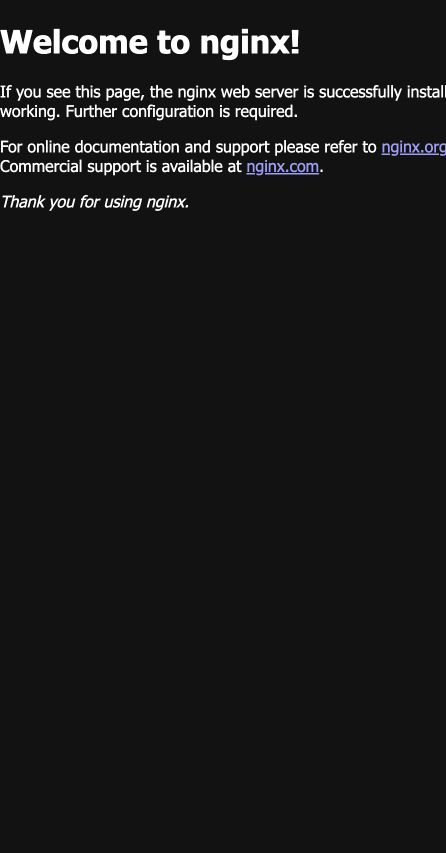
\includegraphics[width=.38\textwidth]{practicas/P05/evidencias/kubernetes.jpg}
\caption{Nginx expuesto mediante el Service de Kubernetes.}
\end{figure}
\begin{figure}[htbp]
\centering
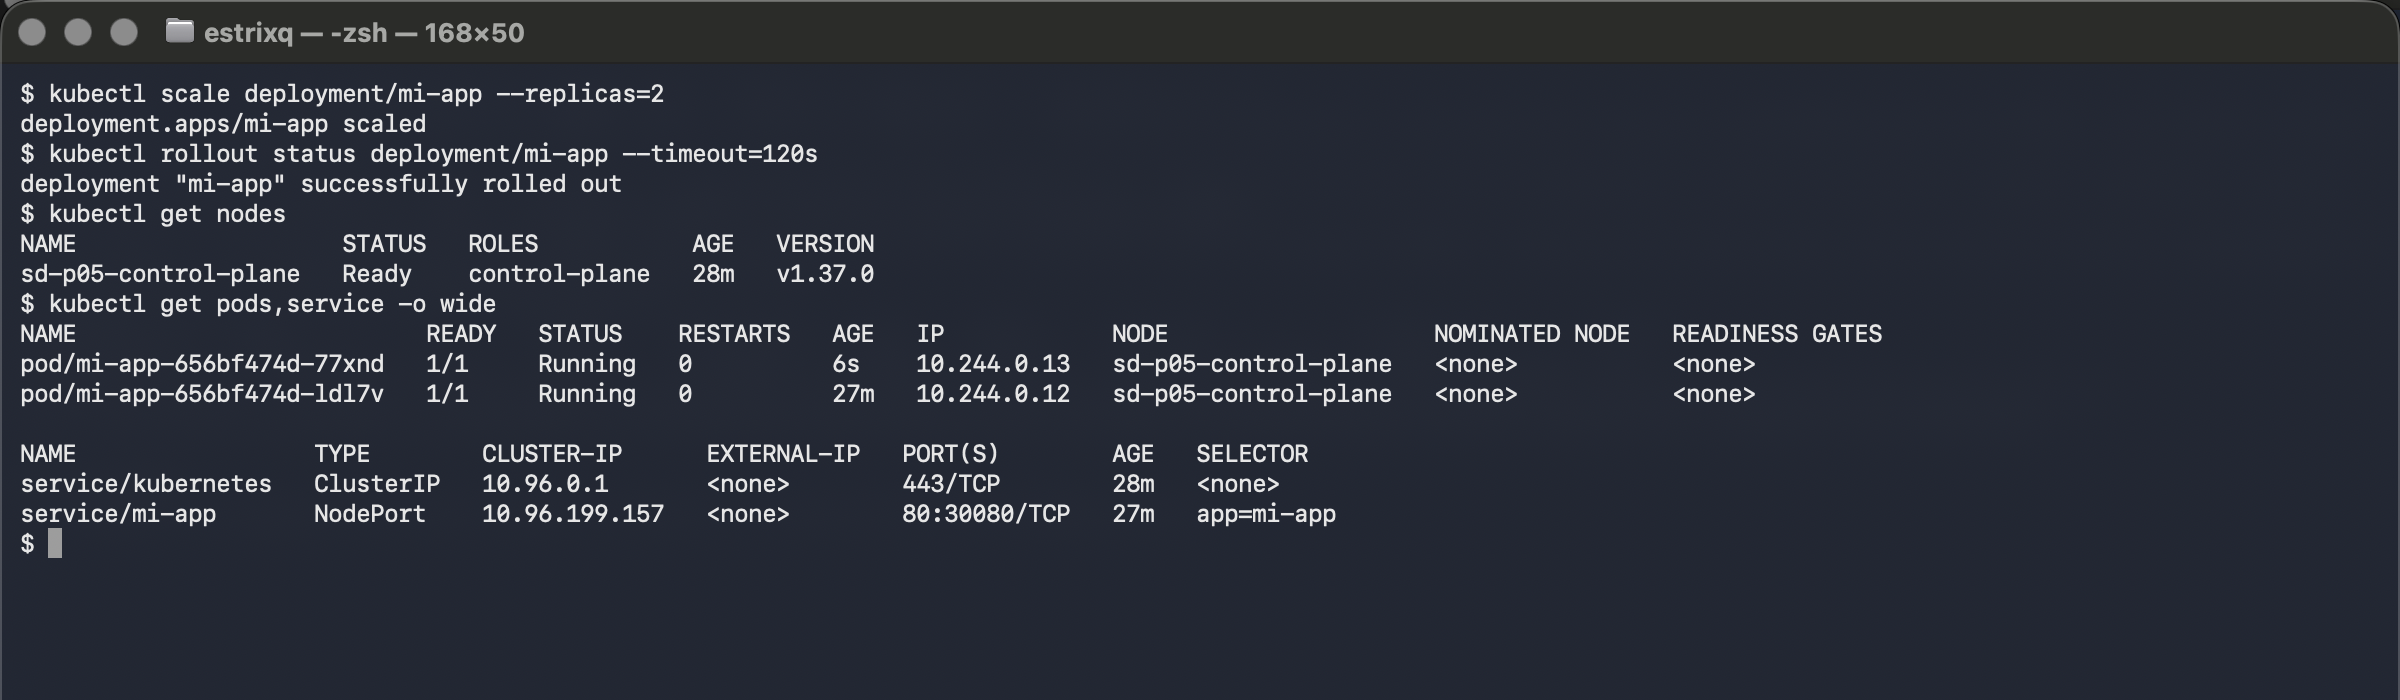
\includegraphics[width=\linewidth]{practicas/P05/evidencias/recortes/kubernetes-2-replicas.png}
\caption{Nodo, Service y dos réplicas iniciales.}
\end{figure}
\begin{figure}[htbp]
\centering
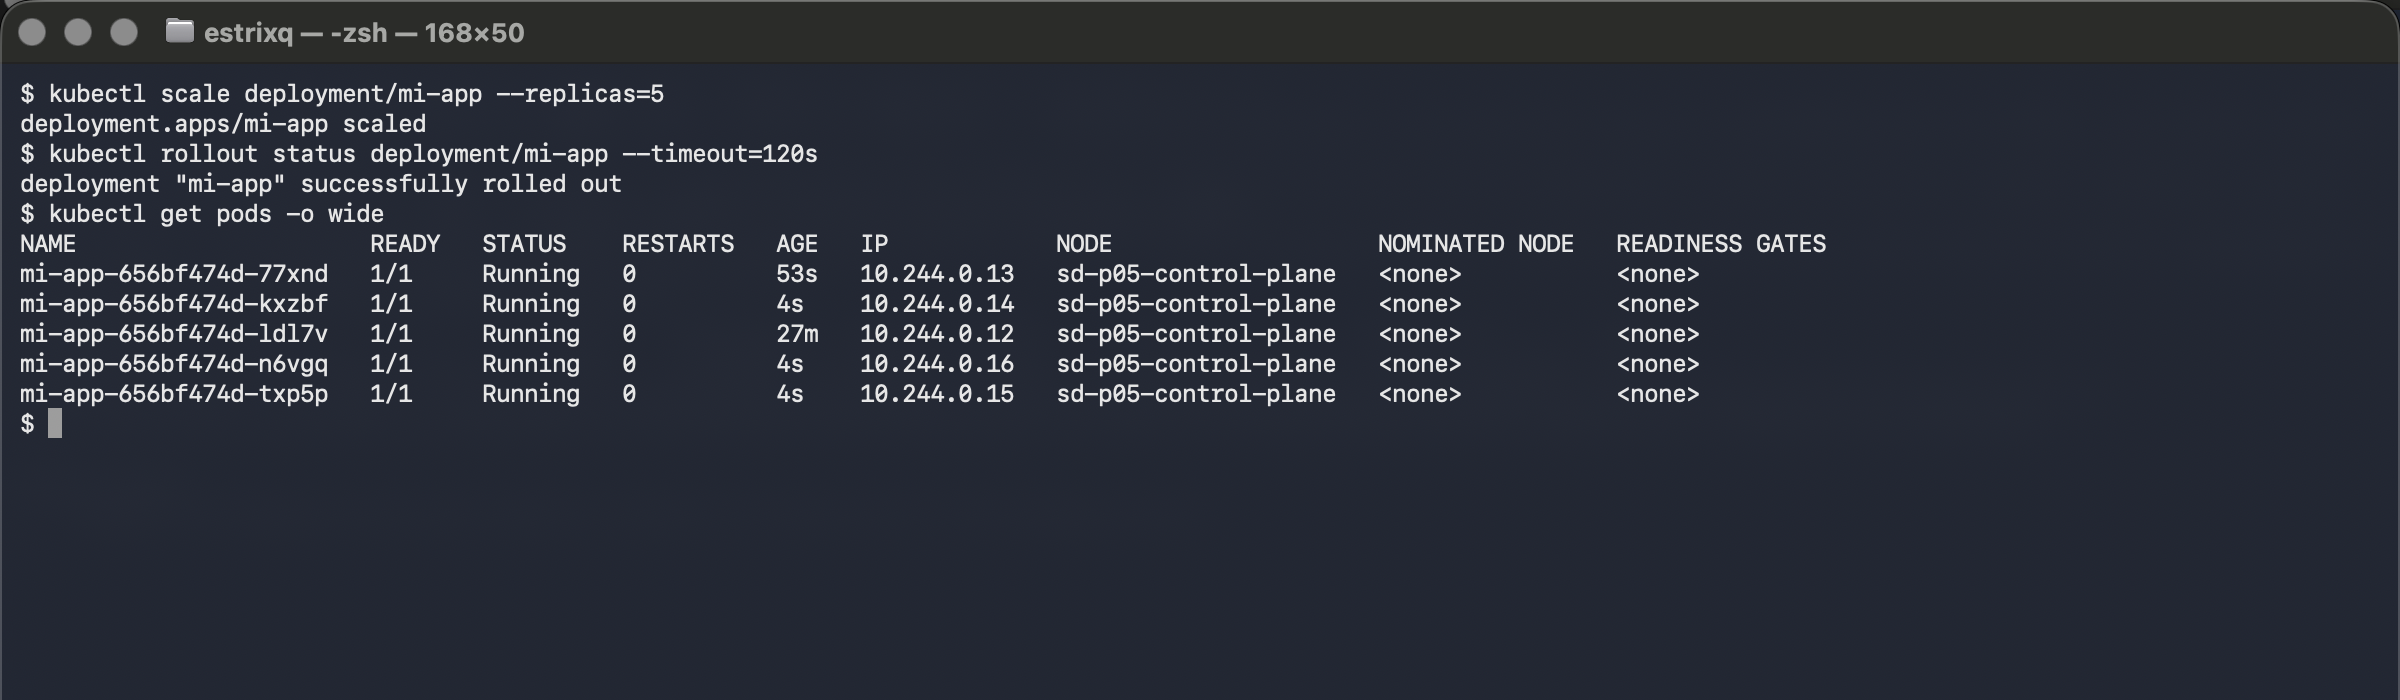
\includegraphics[width=\linewidth]{practicas/P05/evidencias/recortes/kubernetes-5-replicas.png}
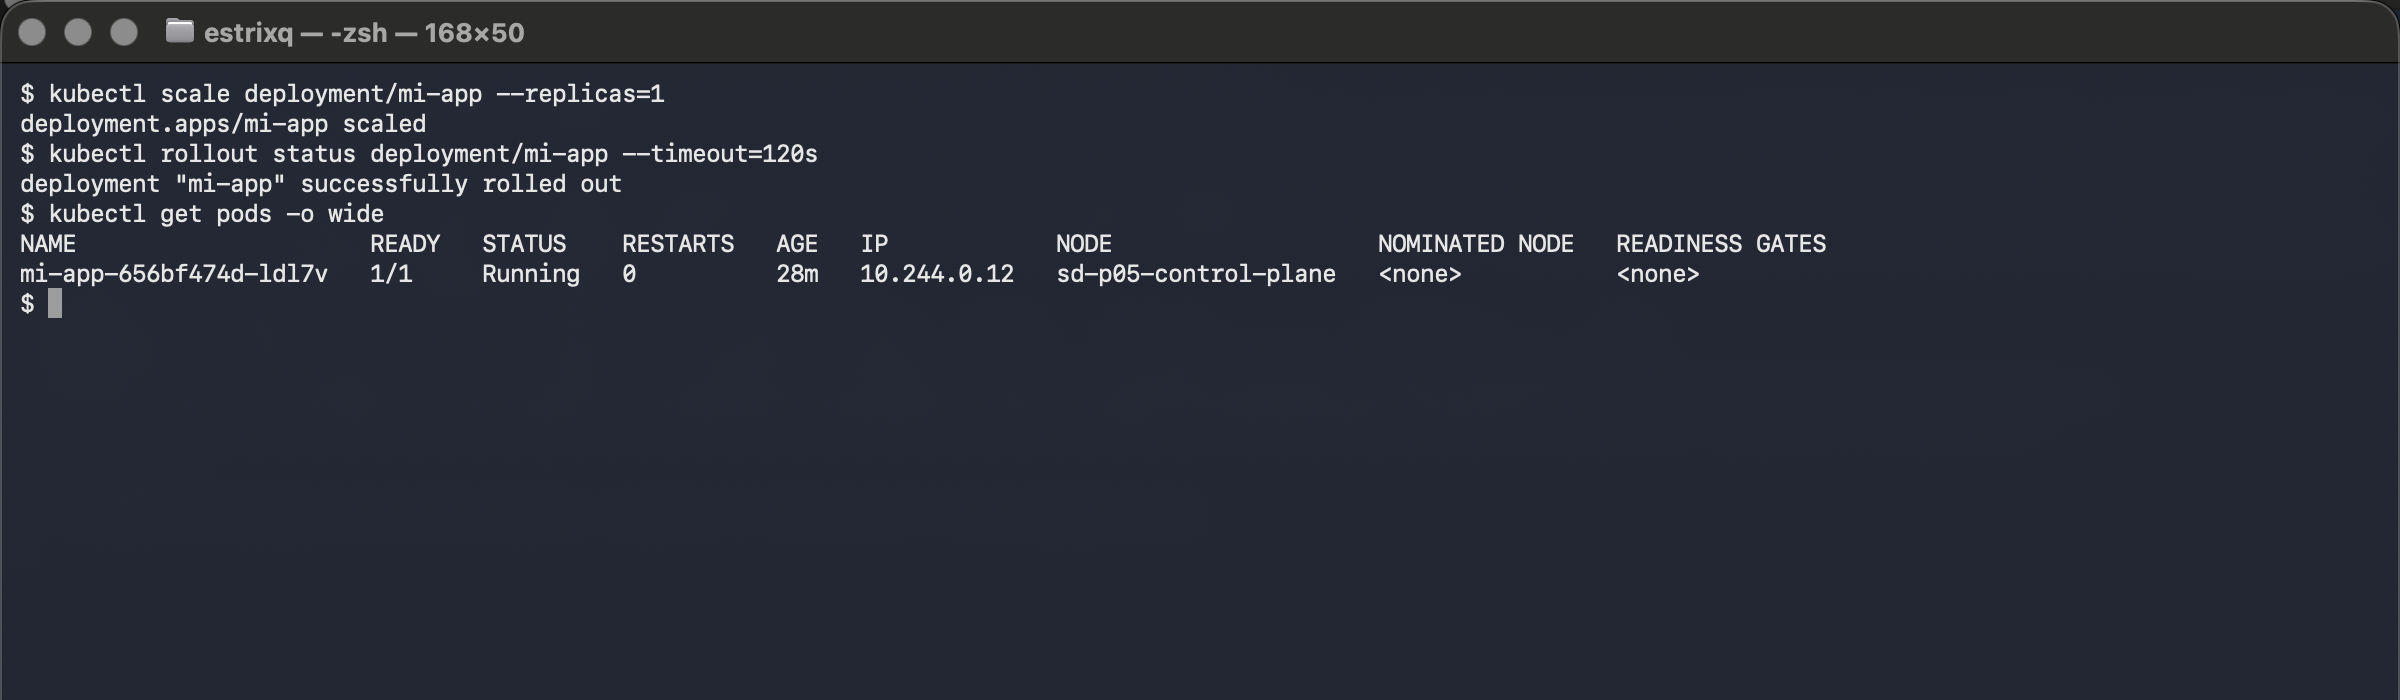
\includegraphics[width=\linewidth]{practicas/P05/evidencias/recortes/kubernetes-1-replica.png}
\caption{Escalado a cinco réplicas y reducción a una.}
\end{figure}

\subsection{Recuperación y actualización}
Después de esperar a que quedara un solo pod activo, se eliminó y se observó la creación de otro. El reemplazo alcanzó la condición \texttt{Ready} en aproximadamente 3 segundos en esta ejecución; el tiempo puede variar. La prueba válida se encuentra en \texttt{evidencias/recuperacion.txt}. Se cambió la imagen de \texttt{nginx:1.25-alpine} a \texttt{nginx:1.27-alpine}, se esperó a que terminara la actualización y se ejecutó un rollback. La imagen final volvió a ser \texttt{nginx:1.25-alpine}.

\begin{lstlisting}[language=bash]
kubectl delete pod <nombre-del-pod>
kubectl set image deployment/mi-app nginx=nginx:1.27-alpine
kubectl rollout status deployment/mi-app
kubectl rollout undo deployment/mi-app
kubectl rollout status deployment/mi-app
\end{lstlisting}

\begin{figure}[htbp]
\centering
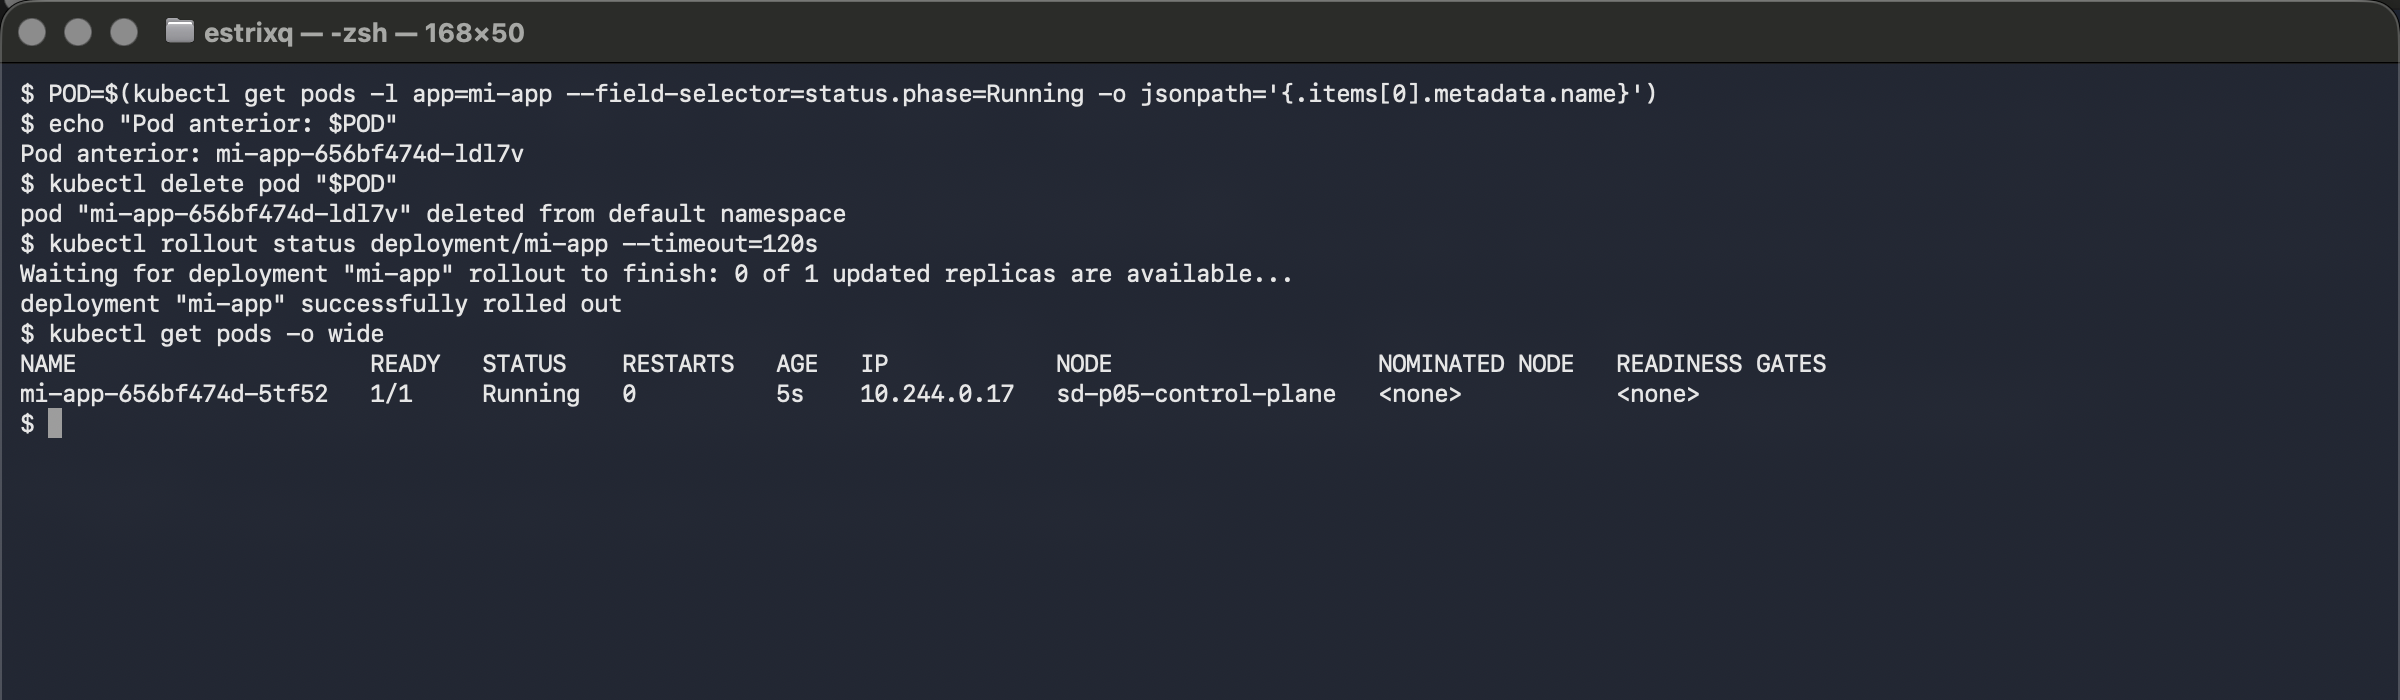
\includegraphics[width=\linewidth]{practicas/P05/evidencias/recortes/kubernetes-recuperacion.png}
\caption{Eliminación y reemplazo de un pod.}
\end{figure}
\begin{figure}[htbp]
\centering
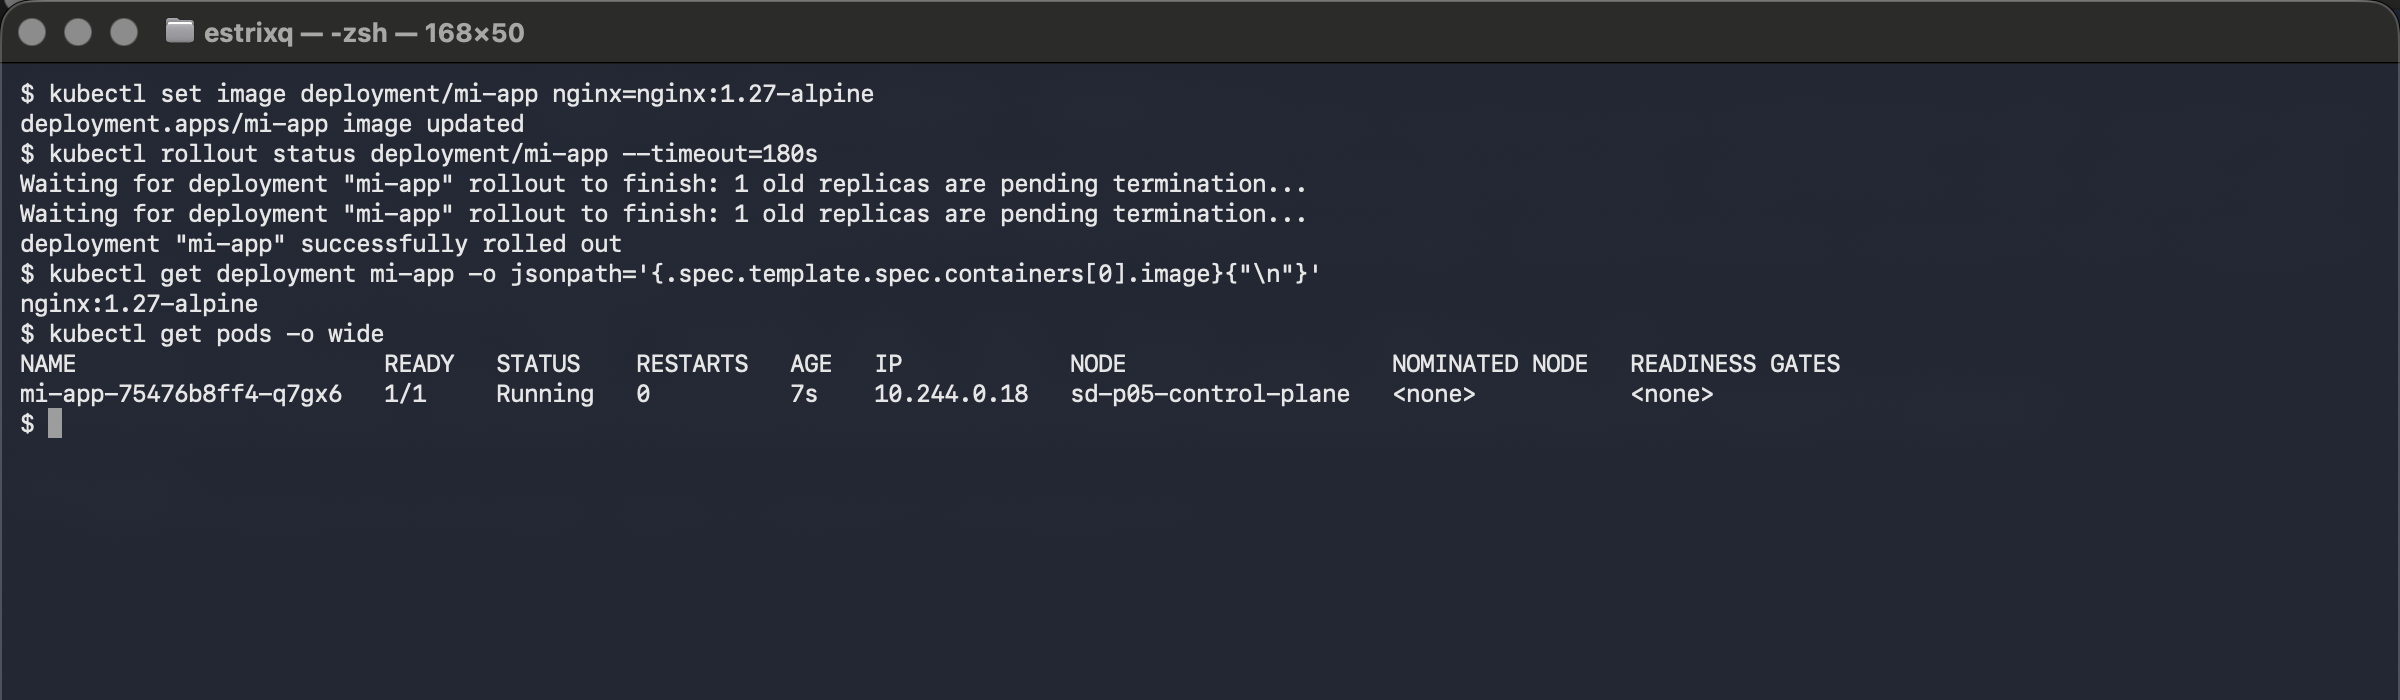
\includegraphics[width=\linewidth]{practicas/P05/evidencias/recortes/kubernetes-actualizacion.png}
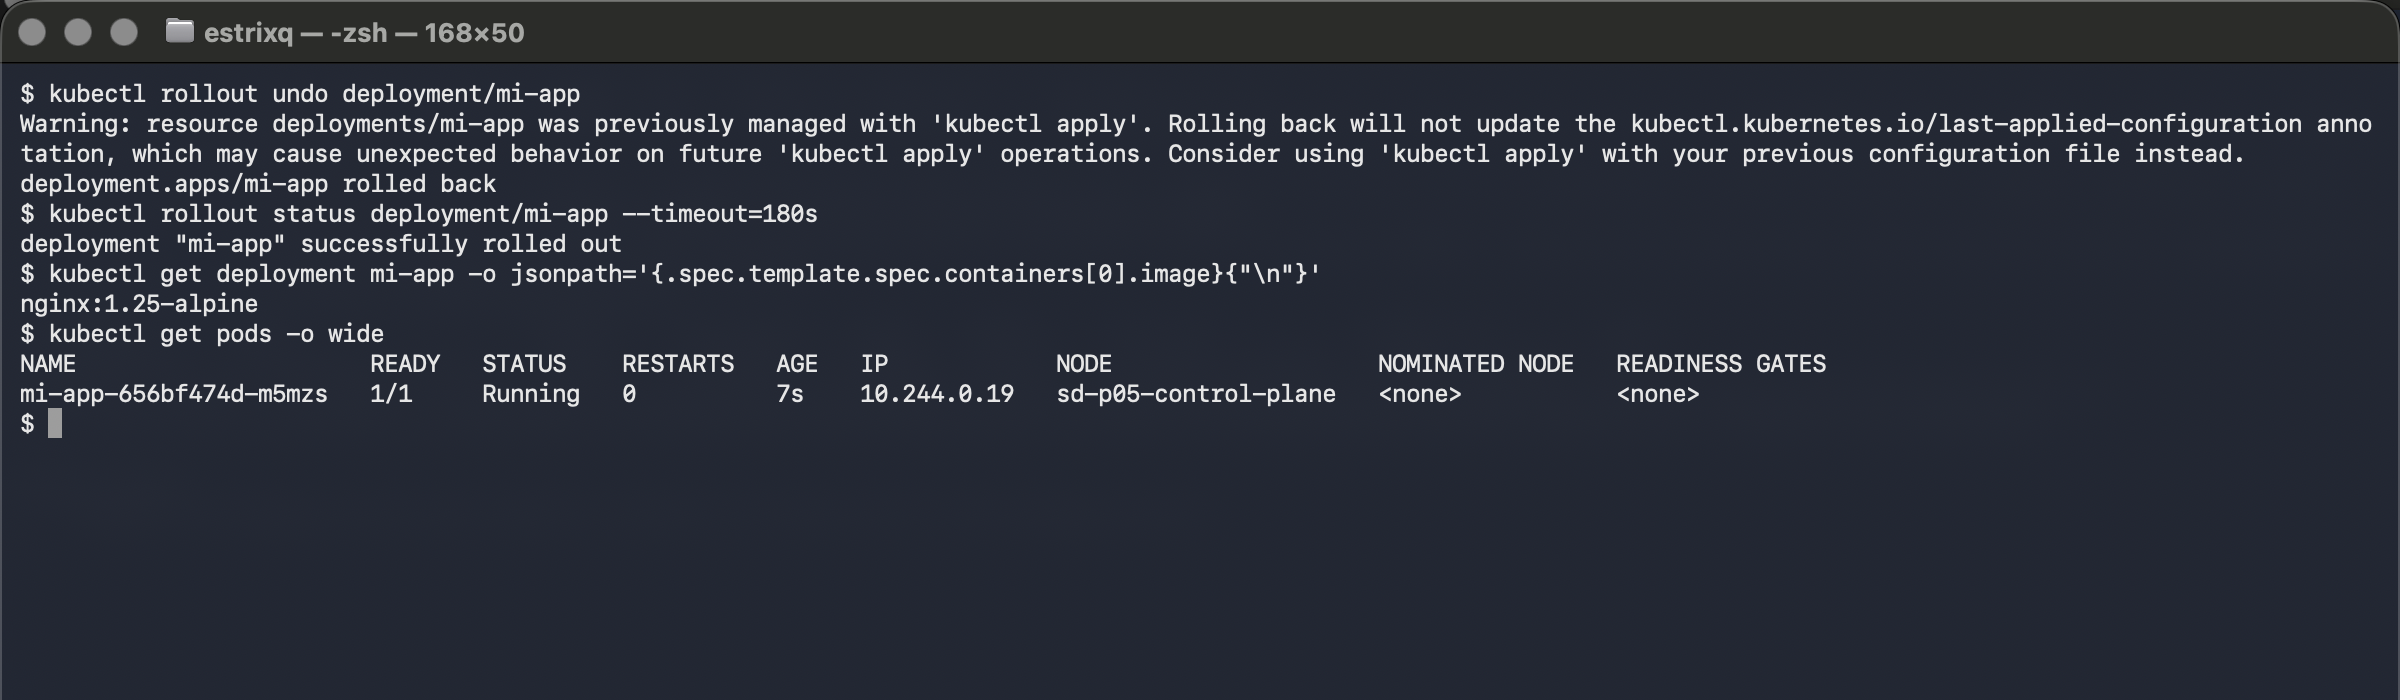
\includegraphics[width=\linewidth]{practicas/P05/evidencias/recortes/kubernetes-rollback.png}
\caption{Actualización de imagen y rollback.}
\end{figure}

\subsection{Preguntas de reflexión}
\begin{enumerate}
\item \textbf{Pod y contenedor.} Un contenedor ejecuta un proceso aislado con su sistema de archivos y dependencias. Un Pod es la unidad mínima de despliegue en Kubernetes y agrupa uno o más contenedores que comparten red y pueden compartir volúmenes. Esta agrupación permite programar juntos procesos estrechamente relacionados, como una aplicación y un contenedor auxiliar.
\item \textbf{Deployment.} Mantiene el número deseado de réplicas mediante ReplicaSets, reemplaza pods que dejan de estar disponibles, permite escalar y administra actualizaciones graduales con posibilidad de rollback. Un Pod creado directamente no proporciona por sí mismo estas funciones de controlador.
\item \textbf{Precios de Kubernetes gestionado.} AKS ofrece una modalidad Free sin cargo de administración del clúster, pero cobra los recursos utilizados y no incluye un SLA financiero de disponibilidad del API; sus modalidades superiores tienen otras condiciones. EKS cobra por hora y por clúster: a USD 0.10 por hora en soporte estándar, 730 horas equivalen a aproximadamente USD 73, además de los recursos de cómputo y red. Son decisiones de precio y servicio de cada proveedor, no una diferencia técnica necesaria. Oracle ofrece OKE Basic Cluster sin cargo por el servicio de clúster; los nodos y demás recursos pueden generar cargos, por lo que no debe suponerse que cualquier configuración sea totalmente gratuita.
\end{enumerate}

\subsection{Referencias}
\begin{itemize}
\item Docker. \href{https://docs.docker.com/engine/security/rootless/}{Rootless mode}.
\item Kubernetes. \href{https://kubernetes.io/docs/concepts/workloads/controllers/deployment/}{Deployments}.
\item Microsoft. \href{https://learn.microsoft.com/azure/aks/free-standard-pricing-tiers}{AKS pricing tiers}.
\item AWS. \href{https://aws.amazon.com/eks/pricing/}{Amazon EKS Pricing}.
\item Oracle. \href{https://www.oracle.com/apac/cloud/iaas-paas/}{OCI Kubernetes Engine Basic Clusters}.
\end{itemize}

\subsection{Archivos de configuración}
Las siguientes rutas son relativas a la raíz del repositorio; ajústense si el documento principal está en otra carpeta.
\lstinputlisting[caption={Servicio web y base de datos con Docker Compose}]{practicas/P05/actividad2/compose/docker-compose.yml}
\lstinputlisting[caption={Dockerfile de la aplicación Flask}]{practicas/P05/actividad2/compose/app/Dockerfile}
\lstinputlisting[caption={Aplicación Flask}]{practicas/P05/actividad2/compose/app/app.py}
\lstinputlisting[caption={Dockerfile de una sola etapa}]{practicas/P05/actividad2/multistage/Dockerfile.single}
\lstinputlisting[caption={Deployment de Kubernetes}]{practicas/P05/actividad3/deployment.yaml}
\lstinputlisting[caption={Service de Kubernetes}]{practicas/P05/actividad3/service.yaml}
